%% dmplex_geom.tex
%% Technical documentation of the distributed DMPlex geometry kernel in BioFEM-IA.
%% Self-contained: compile standalone or \input into a larger document.
%% Requires: amsmath, booktabs, listings, xcolor, hyperref, tikz, pgfplots (optional).

\documentclass[11pt]{article}
\usepackage[margin=1.2in]{geometry}
\usepackage{amsmath,amssymb}
\usepackage{booktabs}
\usepackage{array}
\usepackage{xcolor}
\usepackage[T1]{fontenc}
\usepackage{lmodern}
\usepackage{microtype}
\usepackage{hyperref}
\usepackage{listings}
\usepackage{tikz}
\usetikzlibrary{arrows.meta,positioning,fit,backgrounds,shapes}

\definecolor{codebg}{rgb}{0.97,0.97,0.97}
\definecolor{codekey}{rgb}{0.0,0.35,0.65}
\definecolor{codecomment}{rgb}{0.35,0.55,0.35}
\definecolor{codestring}{rgb}{0.65,0.10,0.10}

\lstset{
  language=C,
  backgroundcolor=\color{codebg},
  basicstyle=\ttfamily\small,
  keywordstyle=\color{codekey}\bfseries,
  commentstyle=\color{codecomment}\itshape,
  stringstyle=\color{codestring},
  breaklines=true,
  frame=single,
  framesep=4pt,
  numbers=left,
  numberstyle=\tiny\color{gray},
  numbersep=6pt,
  tabsize=2,
  showstringspaces=false,
  morekeywords={PetscErrorCode,PetscInt,PetscReal,PetscBool,PetscMPIInt,
                PetscSF,PetscSFNode,DM,DMLabel,IBMNodes,FE,
                DMPlexPatchLayout,DMPlexPatchExchange}
}

\title{\textbf{Distributed Geometry Kernel for Loop Subdivision Surfaces}\\
       \large Technical Reference: \texttt{dmplex\_geom.c} --- BioFEM-IA}
\author{Hossein Geshani}
\date{\today}

\begin{document}
\maketitle
\tableofcontents
\newpage

%% ============================================================
\section{Overview}
%% ============================================================

\texttt{dmplex\_geom.c} implements a parallel geometry evaluation pipeline
for triangulated immersed-boundary surfaces discretized with Loop subdivision
stencils.  The mesh is distributed across MPI ranks using PETSc's \textsc{DMPlex}
infrastructure.  Patch stencils that span partition boundaries are handled by
a \textsc{PetscSF} (Star Forest) coordinate exchange that is constructed once
at initialization and reused every geometry iteration.

The module is relevant to large-scale fluid--structure interaction and
immersed-boundary simulations where the surface geometry must be updated
every time step and scalability of the geometry kernel is critical.

\subsection{Motivation for DMPlex}

The legacy implementation evaluates subdivision geometry on a single MPI rank,
making it the dominant serial bottleneck for meshes above roughly 50{,}000 elements.
Distributing the mesh with \textsc{DMPlex} allows each rank to compute geometry
for its own subdomain, with only the coordinates needed for cross-boundary stencils
communicated via an SF broadcast.

%% ============================================================
\section{Background Concepts}
%% ============================================================

\subsection{Loop Subdivision Stencils}

Loop subdivision refines a triangle mesh by inserting new vertices at edge midpoints
and repositioning existing vertices according to a weighted sum of their neighbours.
For a triangle $e$, the geometry at the subdivision limit surface requires coordinates
from a \emph{patch} of up to $k+6$ neighbouring vertices (where $k$ is the valence
of an irregular vertex) or 12 vertices for regular stencils.
These patch indices are precomputed and stored in \texttt{ibm->patch[16*e + i]},
using original vertex indices $\in [0, N_v)$.

\subsection{PETSc DMPlex}

\textsc{DMPlex} represents a mesh as a Directed Acyclic Graph (DAG) of \emph{points}:
cells (height 0), edges (height 1), and vertices (depth 0).  All points on a given
rank share a single flat \emph{chart} $[\texttt{pStart}, \texttt{pEnd})$.

\begin{itemize}
  \item \texttt{DMPlexGetHeightStratum(dm, 0, \&cStart, \&cEnd)} --- returns the
        range of cell point indices.
  \item \texttt{DMPlexGetDepthStratum(dm, 0, \&vStart, \&vEnd)} --- returns the
        range of vertex point indices.
  \item After \texttt{DMPlexDistribute()}, each rank holds an owned subdomain plus
        \texttt{overlap} layers of \emph{ghost} cells and vertices needed for stencil
        evaluation near partition boundaries.
\end{itemize}

\textbf{Labels.}
A \texttt{DMLabel} is an integer-valued map from point indices to arbitrary integers.
Two labels are created before distribution and migrate with the points:
\begin{center}
\begin{tabular}{lll}
\toprule
Label name & Domain & Value \\
\midrule
\texttt{"biofem\_orig\_cell"}   & cell point $c$   & original cell index $e = c - c_\text{start}$ \\
\texttt{"biofem\_orig\_vertex"} & vertex point $v$ & original vertex index $i = v - v_\text{start}$ \\
\bottomrule
\end{tabular}
\end{center}
These labels are the only thread from distributed-DM point indices back to the
global \texttt{IBMNodes} arrays, which are indexed by original indices throughout.

\subsection{PetscSF: Star Forest}
\label{sec:sf}

A \texttt{PetscSF} encodes a one-to-many MPI communication pattern as a bipartite graph:

\begin{itemize}
  \item \textbf{Roots} --- authoritative data.  Each rank declares \texttt{nroots}
        root slots; other ranks' leaves may point to any of them.
  \item \textbf{Leaves} --- remote copies.  Each rank has \texttt{nleaves} leaves,
        each described by a \texttt{PetscSFNode\{rank, index\}} pointing to
        the root that owns the data.
\end{itemize}

The two fundamental operations are:
\begin{align*}
\texttt{PetscSFBcast}:& \quad \text{root} \rightarrow \text{leaf} \quad
  (\text{owner sends, all needing ranks receive}) \\
\texttt{PetscSFReduce}:& \quad \text{leaf} \rightarrow \text{root} \quad
  (\text{contributions accumulated at owner})
\end{align*}

Figure~\ref{fig:sf} illustrates the SF used in this module.

\begin{figure}[h]
\centering
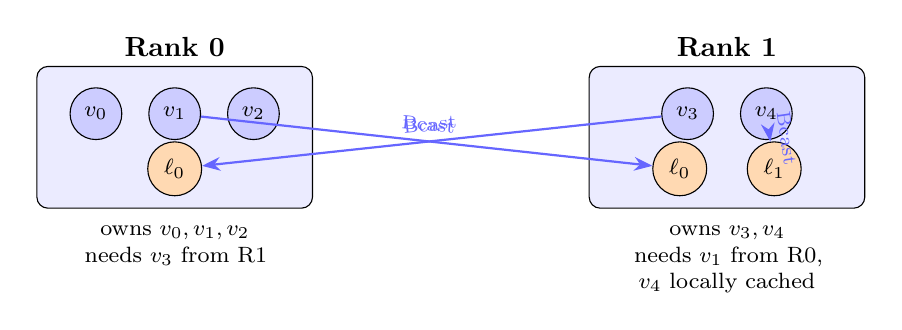
\begin{tikzpicture}[
  rank/.style={draw,rounded corners,minimum width=3.5cm,minimum height=1.8cm,fill=blue!8},
  root/.style={draw,circle,minimum size=0.55cm,fill=blue!20,font=\footnotesize},
  leaf/.style={draw,circle,minimum size=0.55cm,fill=orange!30,font=\footnotesize},
  arr/.style={-{Stealth},thick,blue!60},
  node distance=3.5cm
]
  \node[rank,label=above:\textbf{Rank 0}] (r0box) {};
  \node[rank,right=of r0box,label=above:\textbf{Rank 1}] (r1box) {};

  \node[root] (r0v0) at ([shift={(-1.0, 0.3)}]r0box.center) {$v_0$};
  \node[root] (r0v1) at ([shift={(0.0,  0.3)}]r0box.center) {$v_1$};
  \node[root] (r0v2) at ([shift={(1.0,  0.3)}]r0box.center) {$v_2$};
  \node[leaf] (r0lf) at ([shift={(0.0, -0.4)}]r0box.center) {$\ell_0$};

  \node[root] (r1v3) at ([shift={(-0.5, 0.3)}]r1box.center) {$v_3$};
  \node[root] (r1v4) at ([shift={(0.5,  0.3)}]r1box.center) {$v_4$};
  \node[leaf] (r1lf0) at ([shift={(-0.6,-0.4)}]r1box.center) {$\ell_0$};
  \node[leaf] (r1lf1) at ([shift={(0.6, -0.4)}]r1box.center) {$\ell_1$};

  \draw[arr] (r1v3) -- node[above,sloped,font=\scriptsize]{Bcast} (r0lf);
  \draw[arr] (r0v1) -- node[above,sloped,font=\scriptsize]{Bcast} (r1lf0);
  \draw[arr] (r1v4) -- node[above,sloped,font=\scriptsize]{Bcast} (r1lf1);

  \node[below=0.1cm of r0box,font=\footnotesize,text width=3.5cm,align=center]
    {owns $v_0,v_1,v_2$\\needs $v_3$ from R1};
  \node[below=0.1cm of r1box,font=\footnotesize,text width=3.5cm,align=center]
    {owns $v_3,v_4$\\needs $v_1$ from R0, $v_4$ locally cached};
\end{tikzpicture}
\caption{Star Forest for coordinate exchange.  Blue circles are roots (owned vertices);
orange circles are leaves (remote coordinates needed by this rank's patch stencils).
Arrows show the Bcast direction.}
\label{fig:sf}
\end{figure}

\textbf{Two distinct index spaces.}
The SF in this module uses \emph{original vertex indices} as root slots, not
distributed DM chart indices.  The root data array is \texttt{ibm->x\_bp[0..N\_v)}
and a leaf pointing to \texttt{\{rank $r$, index $i$\}} fetches
\texttt{ibm->x\_bp[$i$]} from rank $r$.  The DM is used only during setup
to determine ownership; once the SF is built, the DM is no longer needed.

%% ============================================================
\section{Data Structures}
%% ============================================================

\subsection{\texttt{DMPlexPatchLayout}}

Per-rank local copy of subdivision stencil data.  All arrays are indexed by
local cell index $\ell_c \in [0, N_\text{local})$.

\begin{center}
\begin{tabular}{lll}
\toprule
Field & Size & Description \\
\midrule
\texttt{dm}        & ---                     & Ref-counted distributed DM. \\
\texttt{orig\_cell}& $N_\text{local}$        & Original cell index $e$ for $\ell_c$; $-1$ for ghosts. \\
\texttt{ire}       & $N_\text{local}$        & 0 = regular stencil, 1 = irregular. \\
\texttt{irv}       & $N_\text{local}$        & Irregular-vertex flag. \\
\texttt{val}       & $N_\text{local}$        & Valence of the irregular vertex. \\
\texttt{patch}     & $16 \times N_\text{local}$ & Original vertex indices of the stencil.
                                               Unused slots: \texttt{PATCH\_MISSING}. \\
\texttt{cStart, cEnd} & ---                  & Cell chart range. \\
\texttt{nLocalCells}  & ---                  & $N_\text{local} = \texttt{cEnd} - \texttt{cStart}$. \\
\bottomrule
\end{tabular}
\end{center}

\subsection{\texttt{DMPlexPatchExchange}}

Holds the SF and coordinate receive buffers.  All arrays indexed by remote node $i
\in [0, N_\text{remote})$.

\begin{center}
\begin{tabular}{lll}
\toprule
Field & Size & Description \\
\midrule
\texttt{sf}           & ---              & PetscSF: $N_v$ roots, $N_\text{remote}$ leaves. \\
\texttt{nRemoteNodes} & ---              & $N_\text{remote}$: unique cross-rank vertices needed. \\
\texttt{orig\_node}   & $N_\text{remote}$ & Original vertex index of remote node $i$. \\
\texttt{owner\_rank}  & $N_\text{remote}$ & MPI rank owning \texttt{orig\_node[$i$]}. \\
\texttt{owner\_index} & $N_\text{remote}$ & Root slot on owner (= \texttt{orig\_node[$i$]}). \\
\texttt{x\_remote}    & $N_\text{remote}$ & Receive buffer for $x$ coordinates. \\
\texttt{y\_remote}    & $N_\text{remote}$ & Receive buffer for $y$ coordinates. \\
\texttt{z\_remote}    & $N_\text{remote}$ & Receive buffer for $z$ coordinates. \\
\bottomrule
\end{tabular}
\end{center}

%% ============================================================
\section{Setup Pipeline}
%% ============================================================

The one-time setup is orchestrated by \texttt{RunDMPlexGeomProcesses()} and
consists of four sequential steps, illustrated in Figure~\ref{fig:pipeline}.

\begin{figure}[h]
\centering
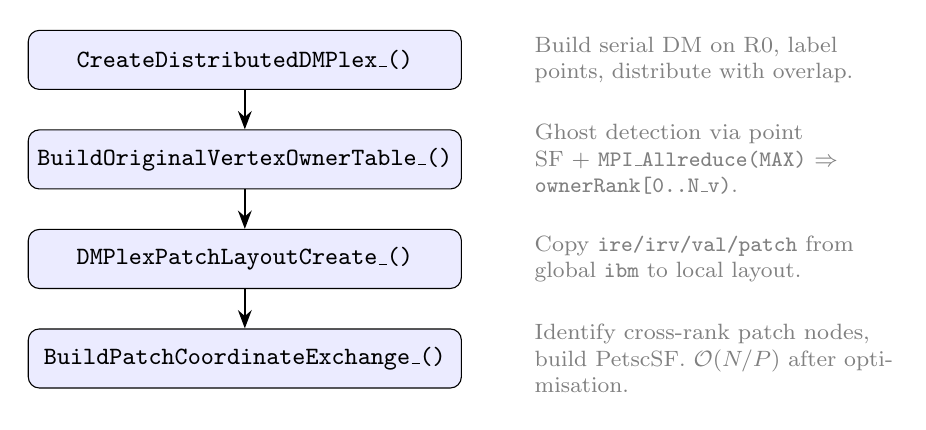
\begin{tikzpicture}[
  box/.style={draw,rounded corners,fill=blue!8,minimum width=5.5cm,
              minimum height=0.75cm,font=\small,align=center},
  arr/.style={-{Stealth},thick},
  note/.style={font=\footnotesize,text=gray,text width=4.5cm,align=left}
]
\node[box] (s1) {\texttt{CreateDistributedDMPlex\_()}};
\node[box,below=0.5cm of s1] (s2) {\texttt{BuildOriginalVertexOwnerTable\_()}};
\node[box,below=0.5cm of s2] (s3) {\texttt{DMPlexPatchLayoutCreate\_()}};
\node[box,below=0.5cm of s3] (s4) {\texttt{BuildPatchCoordinateExchange\_()}};

\draw[arr] (s1)--(s2);
\draw[arr] (s2)--(s3);
\draw[arr] (s3)--(s4);

\node[note,right=0.8cm of s1] {Build serial DM on R0, label points, distribute with overlap.};
\node[note,right=0.8cm of s2] {Ghost detection via point SF + \texttt{MPI\_Allreduce(MAX)} $\Rightarrow$ \texttt{ownerRank[0..N\_v)}.};
\node[note,right=0.8cm of s3] {Copy \texttt{ire/irv/val/patch} from global \texttt{ibm} to local layout.};
\node[note,right=0.8cm of s4] {Identify cross-rank patch nodes, build PetscSF. $\mathcal{O}(N/P)$ after optimisation.};
\end{tikzpicture}
\caption{One-time setup pipeline.}
\label{fig:pipeline}
\end{figure}

\subsection{\texttt{BuildSerialDMPlex\_} and \texttt{LabelOriginalPoints\_}}

Rank 0 fills the cell connectivity and coordinate arrays from \texttt{ibm} and
passes them to \texttt{DMPlexCreateFromCellListPetsc}.
All other ranks pass empty arrays; PETSc collectively constructs the full topology
(including edge interpolation) and holds the complete mesh on rank 0.
\texttt{LabelOriginalPoints\_} then stamps every cell and vertex with its
pre-distribution index, so that after distribution each point on any rank can be
mapped back to the global \texttt{ibm} arrays.

\subsection{\texttt{CreateDistributedDMPlex\_}}

Calls \texttt{DMPlexDistribute(dm, overlap, \&migrationSF, \&distributed)}.
The migration SF is discarded; it was used internally to migrate the labels.
The resulting distributed DM has \texttt{overlap} ghost cell layers on every rank,
which ensures that subdivision stencils of boundary cells can be partially satisfied
by locally available ghost vertex coordinates.

\subsection{\texttt{BuildOriginalVertexOwnerTable\_}}
\label{sec:owner}

The goal is to produce \texttt{ownerRank[i]} = MPI rank that owns original vertex $i$,
globally consistent across all ranks.

\textbf{Step 1: Ghost detection.}
The DM's point SF (\texttt{DMGetPointSF}) records which local points are ghosts.
The SF leaves are exactly the ghost points; their local chart positions are extracted
via \texttt{ilocal} (or the implicit $0,1,2,\ldots$ ordering if \texttt{ilocal == NULL}):
\[
  \texttt{isGhost}[p - p_\text{start}] = \text{true}
  \quad \forall p \in \{\text{SF leaf positions}\}
\]

\textbf{Step 2: Local ownership.}
Iterate over all local vertices $v \in [v_\text{start}, v_\text{end})$, read
\texttt{orig = label(v)}, and for non-ghost vertices set \texttt{localOwner[orig] = myRank}.

\textbf{Step 3: Global reduction.}
\[
  \texttt{ownerRank[i]} = \max_{\text{all ranks}} \texttt{localOwner[i]}
\]
Non-owners contribute $-1$; the owning rank contributes its rank ID $\geq 0$.
\texttt{MPI\_MAX} selects the owner.

\subsection{\texttt{DMPlexPatchLayoutCreate\_}}

Iterates over locally owned cells, reads the \texttt{"biofem\_orig\_cell"} label
to obtain $e$, and copies \texttt{ibm->ire[e]}, \texttt{ibm->irv[e]}, \texttt{ibm->val[e]},
and \texttt{ibm->patch[16e+i]} into the layout arrays.
Ghost cells (label $= -1$) receive \texttt{PATCH\_MISSING} in all patch slots.
This step involves no communication.

\subsection{\texttt{BuildPatchCoordinateExchange\_}}
\label{sec:exchange}

This is the most algorithmically significant step.  It determines which original
vertices this rank needs from others and builds the PetscSF accordingly.

\subsubsection{Naive algorithm (superseded)}

The original implementation called \texttt{OriginalVertexIsLocal\_()}, which scanned
all local vertices $v \in [v_\text{start}, v_\text{end})$ to check whether a given
original vertex index was present:
\[
  \mathcal{O}\!\left(\frac{N_\text{elmt}}{P} \times 16 \times \frac{N_v}{P}\right)
  = \mathcal{O}\!\left(\frac{N^2}{P^2}\right)
\]
A second linear scan (\texttt{IntArrayContains\_}) was used to deduplicate remote nodes.
For $P=32$ and the nx640 mesh ($N_\text{elmt} \approx 612{,}000$, $N_v \approx 307{,}000$),
this produced approximately $3 \times 10^9$ label lookups per rank, causing all
large-mesh jobs to exceed their time limits.

\subsubsection{Optimised algorithm}

Two boolean arrays of size $N_v$ are built in a single $\mathcal{O}(N_v/P)$ walk
before the loop:

\begin{itemize}
  \item \texttt{isLocalOrig[i]}: \texttt{true} iff original vertex $i$ is a non-ghost
        vertex on this rank.  Built by the same ghost-detection walk used in
        \S\ref{sec:owner}, applied to the \texttt{"biofem\_orig\_vertex"} label.
  \item \texttt{alreadyAdded[i]}: deduplication flag; set when vertex $i$ is
        registered in the remote list.
\end{itemize}

The main loop then runs in $\mathcal{O}(N_\text{elmt}/P \times 16)$:

\begin{lstlisting}
for lc in 0..nLocalCells:
    for i in 0..nen:
        node = layout->patch[16*lc + i]
        if MISSING or >= n_v: continue
        if isLocalOrig[node]: continue      // O(1)
        if alreadyAdded[node]: continue     // O(1)
        alreadyAdded[node] = true
        // register as SF leaf
\end{lstlisting}

Table~\ref{tab:complexity} summarises the complexity improvement.

\begin{table}[h]
\centering
\begin{tabular}{lcc}
\toprule
& Naive & Optimised \\
\midrule
Setup walk & $\mathcal{O}(N_v/P)$ & $\mathcal{O}(N_v/P)$ \\
Per patch-node query & $\mathcal{O}(N_v/P)$ & $\mathcal{O}(1)$ \\
Full loop & $\mathcal{O}(N^2/P^2)$ & $\mathcal{O}(N/P)$ \\
Extra memory & 0 & $2 \times N_v$ booleans \\
\bottomrule
\end{tabular}
\caption{Complexity of \texttt{BuildPatchCoordinateExchange\_} before and after optimisation.}
\label{tab:complexity}
\end{table}

\subsubsection{SF construction}

After the loop, a \texttt{PetscSFNode remote[nRemoteNodes]} array is populated with
$\{\texttt{ownerRank}[i],\, i\}$ for each remote node $i$, and the SF is configured:
\begin{lstlisting}
PetscSFSetGraph(sf,
    ibm->n_v,         /* nroots:  full original vertex array */
    nRemoteNodes,     /* nleaves: unique cross-rank vertices */
    NULL,             /* ilocal:  leaves at 0,1,...,nRemoteNodes-1 */
    ...,
    remote,           /* iremote: {rank, origIndex} for each leaf */
    ...);
\end{lstlisting}
Root slots that no leaf points to are never involved in communication.

%% ============================================================
\section{Per-Iteration Kernel}
%% ============================================================

Every geometry update calls two functions:

\subsection{\texttt{UpdatePatchRemoteCoordinates\_}}

Executes three sequential SF broadcasts to fetch updated coordinates of all
cross-rank patch nodes:
\begin{align*}
  \texttt{ibm->x\_bp}[\texttt{orig\_node}[i]] &\leftarrow \texttt{x\_remote}[i] \\
  \texttt{ibm->y\_bp}[\texttt{orig\_node}[i]] &\leftarrow \texttt{y\_remote}[i] \\
  \texttt{ibm->z\_bp}[\texttt{orig\_node}[i]] &\leftarrow \texttt{z\_remote}[i]
\end{align*}
After the write-back, \texttt{ibm->x/y/z\_bp} is consistent on every rank for
all vertices referenced by its stencils.

\subsection{\texttt{RunLocalGeometry\_}}

Loops over locally owned cells and calls:
\begin{enumerate}
  \item \texttt{ElemUpdateGeom0Subdiv} --- reference-configuration geometry.
  \item \texttt{ElemUpdateGeomSubdiv} --- current-configuration geometry.
  \item \texttt{ElemUpdateG} --- metric tensor.
\end{enumerate}
Ghost cells (orig\_cell $<0$ or $\geq N_\text{elmt}$) are skipped.

%% ============================================================
\section{Timing and Benchmarks}
%% ============================================================

\texttt{RunDMPlexGeomProcesses} records wall-clock times (via \texttt{MPI\_Wtime})
for the full setup and for $n_\text{repeat}=3$ geometry kernel iterations.
The first iteration is a cold run (cache effects); subsequent iterations give the
warm steady-state cost.

Selected results from the mesh sweep (GRACE cluster, \texttt{overlap=2}):

\begin{center}
\begin{tabular}{rrccc}
\toprule
$N_x \times N_y$ & $N_\text{elmt}$ & $P$ & Setup (s) & Iter-1 (s) \\
\midrule
$16\times12$   &    334   & 1  & 6.54   & 0.00630 \\
$64\times48$   &  5\,926  & 4  & 275.15 & 0.03583 \\
$64\times48$   &  5\,926  & 32 & 11.49  & 0.00925 \\
$128\times96$  & 24\,132  & 8  & 3375.5 & 0.08660 \\
$128\times96$  & 24\,132  & 32 & 146.6  & 0.02800 \\
$160\times120$ & 37\,846  & 16 & 1527.0 & 0.06090 \\
$256\times192$ & 97\,414  & 32 & 3950.6 & 0.07881 \\
\bottomrule
\end{tabular}
\end{center}

The large setup times at low core counts reflect the $\mathcal{O}(N^2/P^2)$
complexity of the pre-optimisation \texttt{BuildPatchCoordinateExchange\_};
after the fix these collapse to the DMPlex distribution cost.

%% ============================================================
\section{Call Graph Summary}
%% ============================================================

\begin{lstlisting}[language={},numbers=none,frame=none,backgroundcolor=\color{white}]
RunDMPlexGeomProcesses()
  CreateDistributedDMPlex_()
    BuildSerialDMPlex_()          // rank 0 only, serial
    LabelOriginalPoints_()        // rank 0 only, serial
    DMPlexDistribute()            // collective
  BuildOriginalVertexOwnerTable_()
    DMGetPointSF()
    MPI_Allreduce(MPI_MAX)        // collective, size N_v
  DMPlexPatchLayoutCreate_()      // local, no comms
  BuildPatchCoordinateExchange_() // local + PetscSFSetUp()
    [per iteration:]
  RunLocalGeometry_()
    UpdatePatchRemoteCoordinates_()
      PetscSFBcast() x3           // collective
    ElemUpdateGeom0Subdiv()       // local per cell
    ElemUpdateGeomSubdiv()        // local per cell
    ElemUpdateG()                 // local per cell
\end{lstlisting}

%% ============================================================
\section{Runtime Options}
%% ============================================================

\begin{center}
\begin{tabular}{lll}
\toprule
Option & Default & Description \\
\midrule
\texttt{-dmplex\_geom\_overlap} & 2 & Ghost overlap layers for DMPlex distribution. \\
\texttt{-nbody}                 & 1 & Number of IBM bodies to process. \\
\bottomrule
\end{tabular}
\end{center}

A larger overlap increases the fraction of cells whose stencils are fully local
(reducing SF traffic) at the cost of a larger ghost layer.

\end{document}
